%Instruct LaTeX that you would like to format an article and are using a4paper, default is US Letter size!
\documentclass{article}

%Set up a4paper size and sensible margins
\setlength\parindent{0pt}
\usepackage[a4paper]{geometry}

%Include support for graphics! 
\usepackage{graphicx}
\usepackage{amsmath}
\usepackage{subcaption}

%Include support for url linking
\usepackage[hidelinks]{hyperref}



\iffalse
\begin{figure}[h]
\centering
\includegraphics[width=10cm]{flowchart2.png}
\caption{The steps taken in the simulation after defining the constants}
	\label{flowchart2}
\end{figure}
\fi



\iffalse
\begin{figure}
\centering
\begin{subfigure}{.55\textwidth}
  \centering
  \includegraphics[width=.6\linewidth]{thompsontrajectory}
  \caption{Trajectories}
  \label{thompsontrajectory}
\end{subfigure}%
\begin{subfigure}{.55\textwidth}
  \centering
  \includegraphics[width=.6\linewidth]{thompsontheta}
  \caption{The scattering angle is too small}
  \label{thompsontheta}
\end{subfigure}
\caption{Thompson's model}
\label{thompson}
\end{figure}
\fi



\title{Investigation of Muon Tracking at the CMS Detector}
\author{Nikolaos Koukoulekidis \& 00950301 \\ Stefanos Mousafeiris \& 00951054}
\date{\today}

\begin{document}

\maketitle


\begin{abstract}

A simulation of muon trajectories in the CMS detector was constructed in order to examine the performance of the two main detector systems and estimate the Higgs boson mass distribution by detecting its muon decay products. Trajectories were fitted using a least squares regression method on position measurements of the simulated muons made by the detectors. The momentum range of effectiveness for each detector system was established and the mass of the Higgs boson was estimated to be $(124.98\pm0.02)\ GeVc^{-2}$.
\end{abstract}

\section*{Introduction}

The Compact Muon Solenoid (CMS) is a particle detector built on the LHC at CERN. It is designed to detect collisions up to the $TeV$ scale and its general purpose is to explore features of various particles and consequently contribute to the development of aspects of the Standard Model. A major current goal of the CMS is to provide evidence for the existence of the Higgs boson. This elementary particle plays an important role in our understanding of particle physics theory.

\begin{figure}[h]
\centering
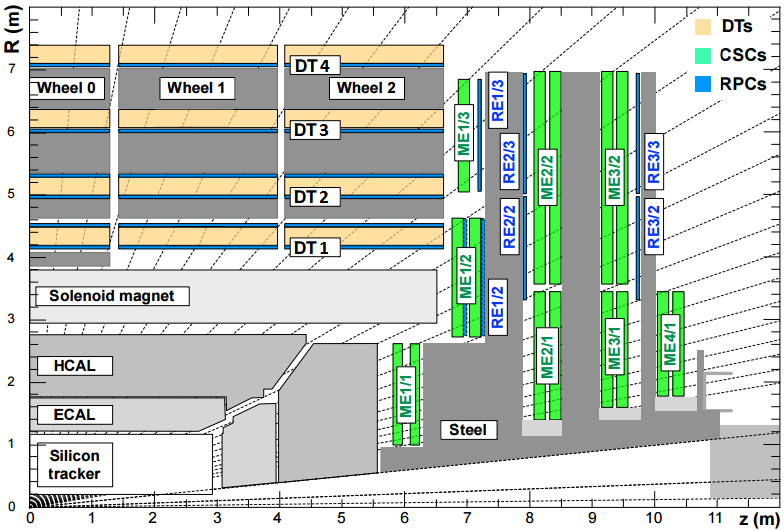
\includegraphics[width=11cm]{cmslayout.png}
\caption{An $r-z$ cross section of a quadrant of the CMS~\cite{cms}.}
	\label{cmslayout}
\end{figure}

Our investigation focuses on the detection of muons resulting from particle collisions.  Figure \ref{cmslayout} illustrates the main parts the CMS consists of. Collisions occur around the origin within the silicon tracker. The resulting muon products travel through the silicon tracker, hadronic calorimeter (HCAL), and drift tubes (DTs) and interact with them. Silicon trackers and DTs contain cylindrical detectors that record the position of the muons when they cross them (hit points). We ignore the detectors vertical to the z-axis as they do not contribute to the purpose of the investigation.\\

This investigation consisted of simulating muon trajectories in the CMS in order to estimate momentum measurements taken by the aforementioned detector systems. The aim  was to compare the effective resolution of the measurements between the silicon tracker and the DT detectors. Consequently, estimates of the mass distribution of the Higgs and $Z$ bosons were made by simulating a Higgs decay into muons.



\section*{Theory}

The Higgs boson $H$ can decay into one on-shell $Z$ and one off-shell $Z^*$ bosons. The off-shell boson has a smaller mass than the on-shell so as to add up to the Higgs mass. Both bosons further decay into a muon $\mu^-$ and an anti-muon $\mu^+$.

\begin{align}
&H \rightarrow ZZ^* \rightarrow \mu^+\mu^-\mu^+\mu^- \label{higgsdecay}
\end{align}
The muon products are then detectable in the CMS.\\

Such a muon travels within the magnetic field of the solenoid magnet in the CMS. The magnetic field lines lie along the z axis and are directed as in figure \ref{muonpath} and the muon paths are hence curved in the $r-\phi$ plane. The field is assumed to have constant magnitude throughout the CMS.

\begin{figure}[h]
\centering
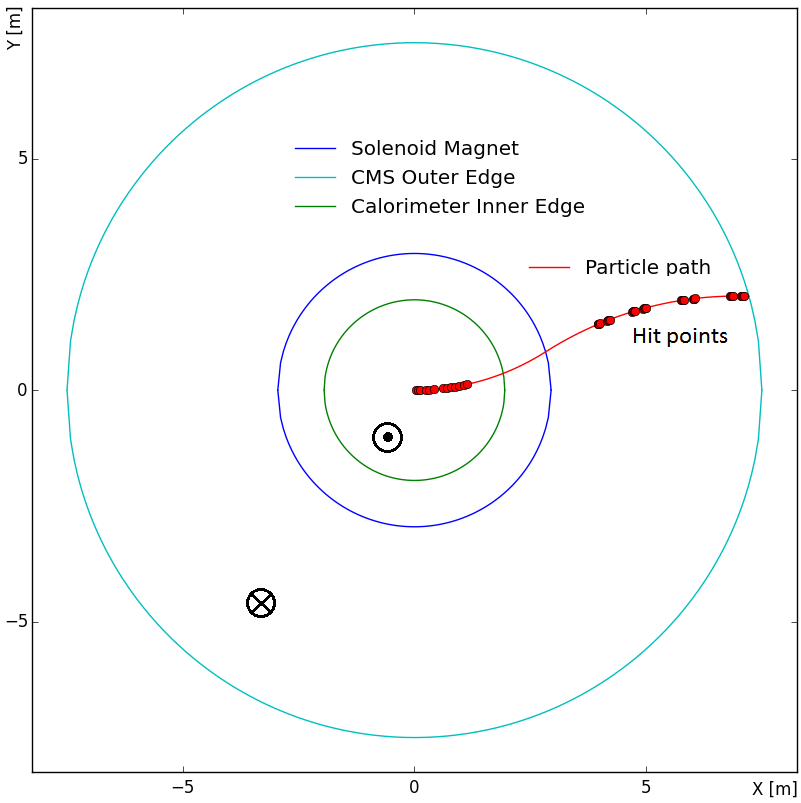
\includegraphics[width=7.23cm]{muonpath.png}
\caption{An $r-\phi$ cross section of a simulated path of a muon produced by a decay at the origin. The black arrows indicate the direction of the magnetic field inside and outside of the magnet.}
	\label{muonpath}
\end{figure}

The muon has an initial momentum due to the decay process which determines its path through the detectors. Therefore, these muons follow helical paths with the curvature of the path changing when they pass from the silicon tracker into the drift tubes.\\

The HCAL lies at the end of the silicon tracker, after the detectors. Only particles with very high momentum can pass through it and into the DT system. The muons are simulated to experience a normal random energy loss as a function of the distance travelled in the calorimeter with an average rate value of $\left< \frac{dE}{dx} \right> = (1.5 \pm 0.5)\ GeVm^{-1}$. Although this loss is accounted for in the result by a systematic correction corresponding to the average energy loss, the muon trajectories are slightly altered before crossing the DT detectors.\\

The initial momentum of the muon in units of $GeVc^{-1}$ is given by
\begin{align}
&p=0.3Br,\label{curvature}
\end{align}
where the magnetic field $B$ is $5T$ and $3.8T$ in the silicon tracker and the DTs respectively, while $r$ is the radius of curvature of the path. Since there is a correction for the calorimeter this equation holds for the DTs as well as the silicon tracker, although the calorimeter will insert some further random uncertainty to the DT system which is not a factor for the silicon tracker detectors.\\

Relativistic momentum and energy conservation lead from the mass and momentum of the muons to mass distributions for the bosons that produced them.

\section*{Method}

The first part of the simulation involved exploring possible muon trajectories in the CMS. The following flowchart describes the steps taken towards producing meaningful data.

\begin{figure}[h]
\centering
\includegraphics[width=10.7cm]{flowchart2.png}
\caption{The algorithm used to produce data for the muon momentum.}
	\label{flowchart}
\end{figure}

A virtual muon was given an initial position around the origin and an initial momentum in the range of $0 - 7000\  GeV$ in order to create a perfect trajectory with a certain radius of curvature and produce hit points by crossing the detectors. The momentum range considered corresponds to realistic momenta observed in the CMS. The detector arrangement used consisted of 13 and 32 hit points in the silicon tracker and the DTs respectively.\\

Randomising the hit points implies the creation of new hit points at each detector via a Gaussian distribution centred at the recorded perfect hit point with a standard deviation corresponding to the intrinsic resolution of the individual detector. The intrinsic resolution was modelled to be generally lower the further the detector lies from the origin, with the silicon tracker and DT detectors producing a standard deviation of the order of $10^{-5}$ and $10^{-4}$ metres respectively. However, the hit points in the DTs are more in number and more spread out as seen in figure \ref{muonpath}. All these facts affected the fitting for different momenta. Particularly the transverse component of the momentum, i.e. the component on the $r-\phi$ plane, was largely affected due to the curvature of the path on that plane, while the $z$ component was relatively unaffected. Therefore, most of the discussion concerns the ability of the detectors to resolve the transverse component of momentum.\\

The helical path was fitted using a least-squares regression method.
Iterations always involved re-randomisation of the hit points which caused the rest of the process to repeat. The results were used to compare the momentum resolution of the silicon tracker and the DT detectors.\\

Eventually, a large dataset of simulated muons was used to estimate the Higgs and $Z$ bosons' mass distributions by measuring the momentum of the muons using the aforementioned process. This involved determining which detector system is best to use for different muon momenta according to the previous analysis. All muons were assumed to be products of Higgs decays and care was taken to choose the correct muon pairs so that an on-shell and an off-shell $Z$ boson were created for each decay.

\section*{Results}

Some special cases of muons with different inital momenta were initially analysed to establish a conjecture for the detector behaviour. The first case is the case of a low energy muon.

\begin{figure}[h]
\centering
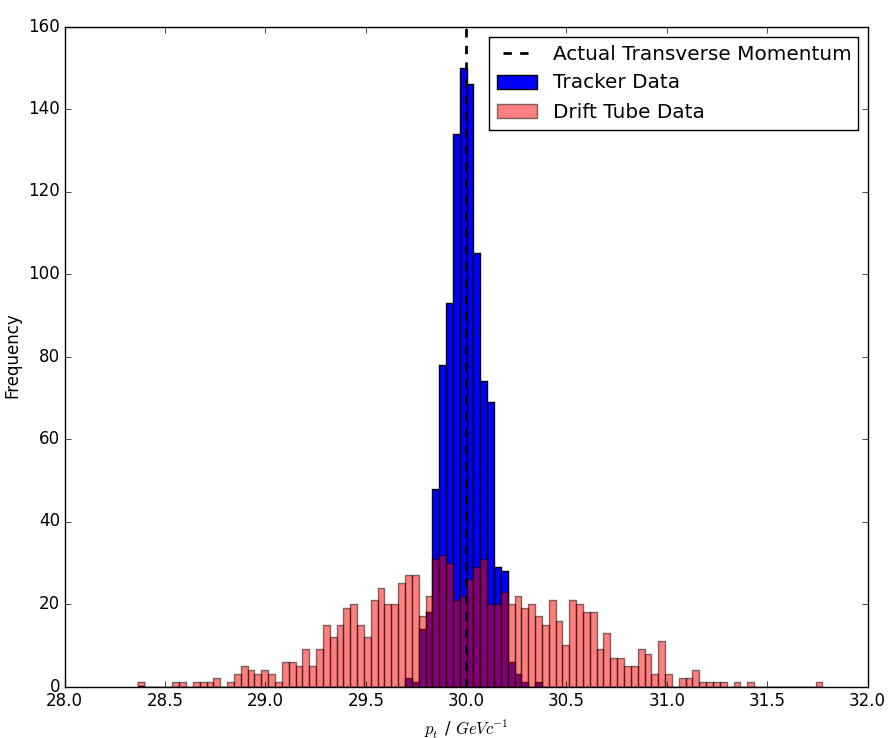
\includegraphics[width=12.1cm]{pt30.png}
\caption{A histogram of the momentum distribution for a low energy muon ($p_t=30\ GeVc^{-1}$).}
	\label{pt30}
\end{figure}

Both the silicon tracker and the DTs produce normally distributed measurements centred around approximately $30\ GeVc^{-1}$. Since the simulated muon was given a momentum of exactly $30\ GeVc^{-1}$, both distributions can be considered accurate. The main reason is that a low energy muon trajectory has a high curvature as seen in equation \ref{curvature} and a helical path can be accurately fitted. The silicon tracker distribution exhibits a lower standard error, i.e. a more narrow spread, than the DT distribution. Since the energy of the muon is comparable to the average energy loss due to the HCAL, the random variations of that loss had a significant impact on the resolution. The higher intrinsic resolution of the individual detectors in the silicon tracker was not found to greatly affect the effective resolution.\\

The second case is the case of a `critical' energy muon.

\begin{figure}[h]
\centering
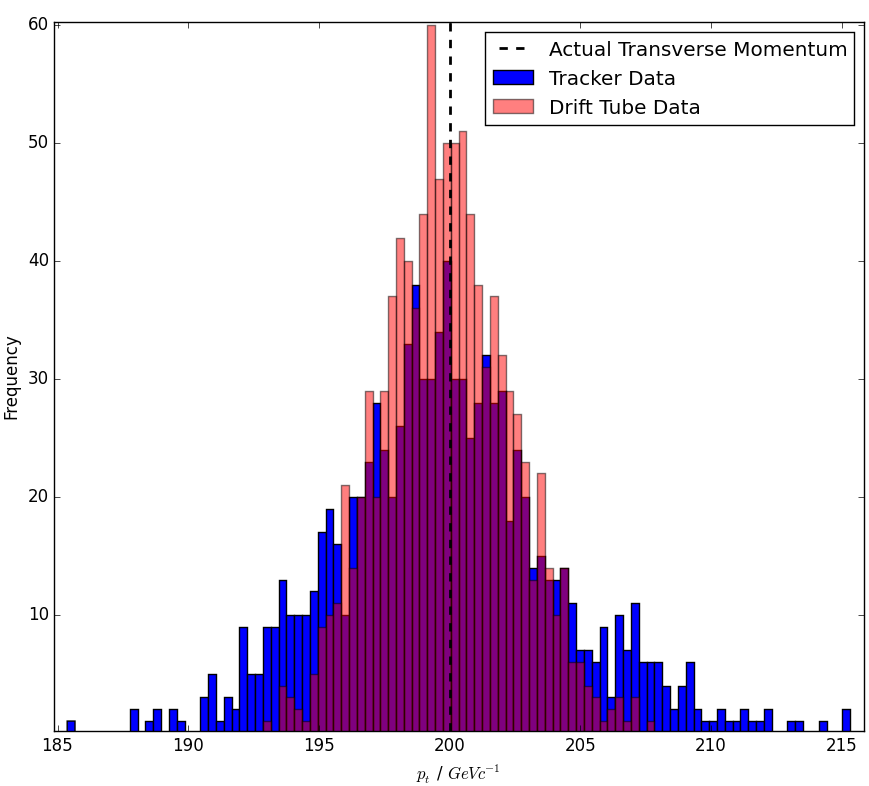
\includegraphics[width=13cm]{pt200.png}
\caption{A histogram of the momentum distribution for a `critical' energy muon ($p_t=200\ GeVc^{-1}$).}
	\label{pt200}
\end{figure}

Both the silicon tracker and the DTs produce normally distributed measurements centred around approximately $200\ GeVc^{-1}$. Since the simulated muon was given a momentum of exactly $200\ GeVc^{-1}$, both distributions can be still considered accurate. At these energy levels, the average energy loss is significantly lower than the energy of the simulated muons and therefore the spread of the DT distribution becomes comparable with the spread of the silicon tracker distribution.\\

A third case is the extreme case of a very high energy muon.

\begin{figure}[h]
\centering
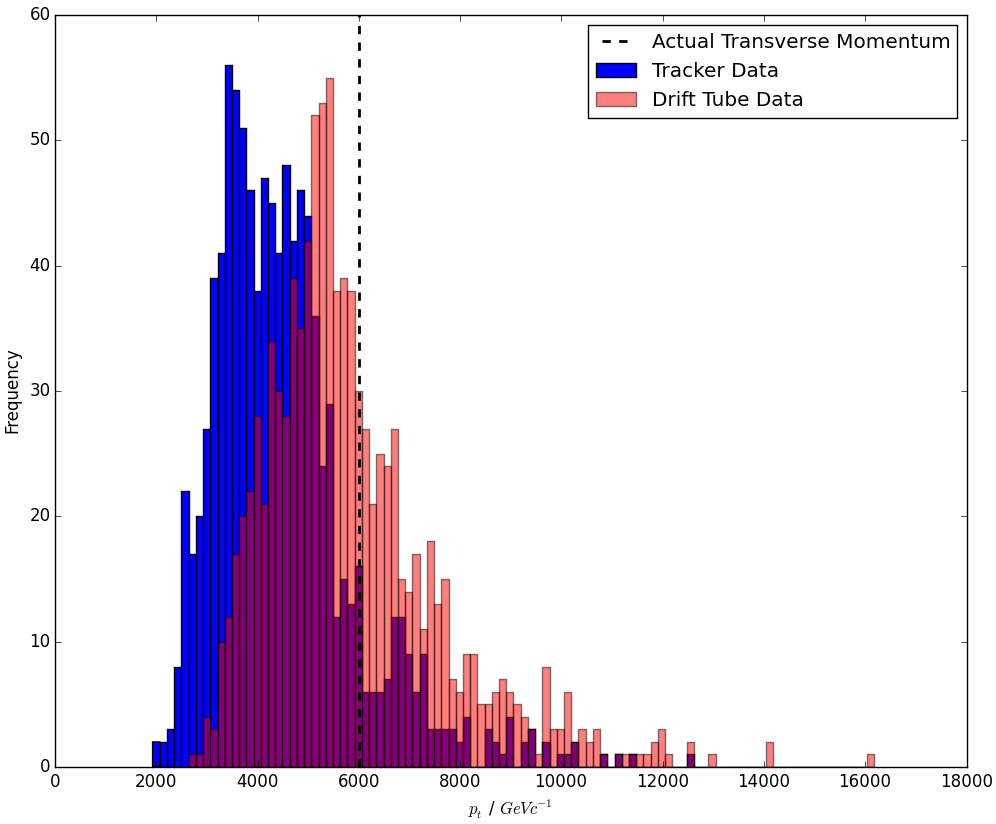
\includegraphics[width=13cm]{pt6000.png}
\caption{A histogram of the momentum distribution for a very high energy muon ($p_t=6000\ GeVc^{-1}$).}
	\label{pt6000}
\end{figure}

At such high energy levels, both momentum distributions are skewed to the right and their peaks are shifted left of the simulated muon’s momentum. The path of muons approximate straight lines at high momenta and therefore fitting a helical path involves a very high error as seen by the very large spread.\\

The above graphs suggest trends for the accuracy and precision of the momentum measurements depending on the observed momentum range.\\

In figure \ref{errors} the effective resolution of the tracker is observed to worsen linearly as momentum increases. This is mainly because of the difficulty encountered when fitting a helical path as the path straightens for higher momenta.

\pagebreak

\begin{figure}[h]
\centering
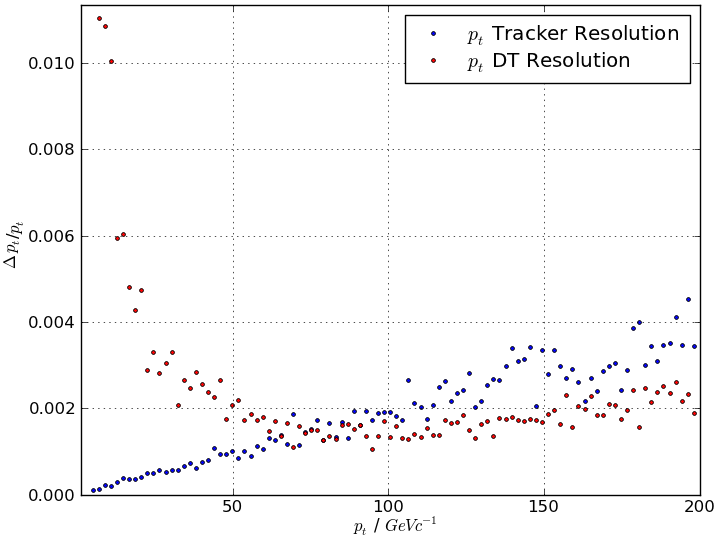
\includegraphics[width=13cm]{errors.png}
\caption{A plot of the effective resolution of the silicon tracker and DT detector systems against muon momentum.}
	\label{errors}
\end{figure}

The effective resolution of the DT system is improving as momentum increases in the beginning. This happens due to the lesser impact of the HCAL on the shift of the muon's trajectory. However, the DT resolution overtakes the silicon tracker resolution and remains relatively constant within the interval $80 - 100\ GeVc^{-1}$ at which the difficulty to fit a helical path starts becoming more significant than the lessening impact of the HCAL. After this interval the resolution follows the trend of the silicon tracker with a lower slope, so that the DT resolution is always better than the silicon tracker resolution.\\

The range of momenta in figure \ref{errors} was chosen so as to include only low values of momentum for which the detector systems are sufficiently accurate. Beyond that range, the accuracy tends to decrease as seen in figure \ref{pt6000} for the extreme cases. The accuracy of the detectors was examined by plotting the fractional deviation of the measured momentum from the simulated muon's momentum against the latter as in figure \ref{deviations}.

\pagebreak

\begin{figure}[h]
\centering
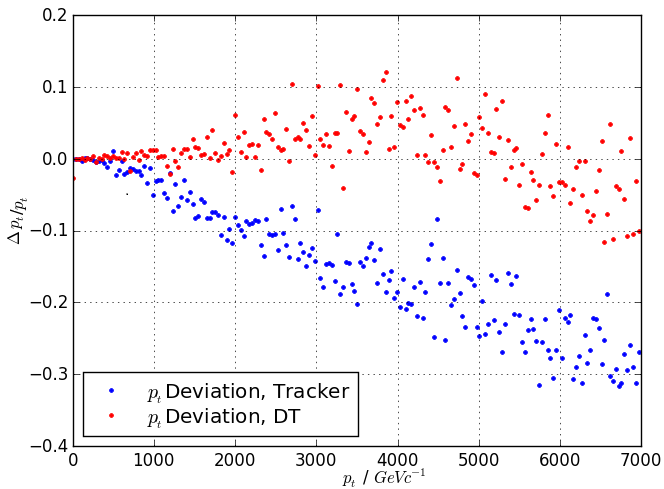
\includegraphics[width=13cm]{deviations.png}
\caption{A plot of the momentum deviation of the silicon tracker and DT detector systems against muon momentum.}
	\label{deviations}
\end{figure}

In the range of low momenta, the deviation is very close to zero and thus the effective resolution essentially depends on the precision, as previously discussed. Beyond the value of approximately $400\ GeVc^{-1}$ the deviation of the silicon tracker system starts to increase in a linear fashion reaching a $30\%$ underestimation at the extreme case of $7\ TeVc^{-1}$.\\

The DT system deviation oscillates between positive and negative values, but always remains within $10\%$. It also seems to always have a value closer to zero than the deviation of the silicon tracker system of detectors. Therefore, the DT system is expected to yield more reliable measurements of high momentum muons as seen in figure \ref{pt6000} as well.\\

The reason behind the constant underestimation by the silicon tracker detectors and the oscillatory behaviour of the DT system accuracy was attributed to the fitting function by a process of trial and error. It was conjectured that at high momenta the radius of curvature calculated from the fitting tends to remain constant because the change in the curvature of the trajectory is nearly indistinguishable. Therefore, the radius, and hence the momentum, is increasingly underestimated explaining the tracker detectors' behaviour and the behaviour of the DT system beyond the peak in deviation at approximately $4000\ GeVc^{-1}$. The initial overestimation of the DT system before the peak is considered unimportant given the dispersion of the data in figure \ref{pt6000}.\\

\pagebreak

Eventually, the mass distribution of a Higgs and two $Z$ bosons were plotted by simulating a Higgs decay into four muons described by equation \ref{higgsdecay}.\\

Figure \ref{zbosons} illustrates the resulting mass distributions of the $Z$ bosons. The distribution of the on-shell $Z$ boson approximates a Gaussian distribution with a mean value of $91\ GeVc^{-2}$ with a standard error of $1\ GeVc^{-2}$. The off-shell boson also seems to have a normal mass distribution with a mean value of $30\ GeVc^{-2}$ and a larger associated error of $5\ GeVc^{-2}$.\\

\begin{figure}[h]
\centering
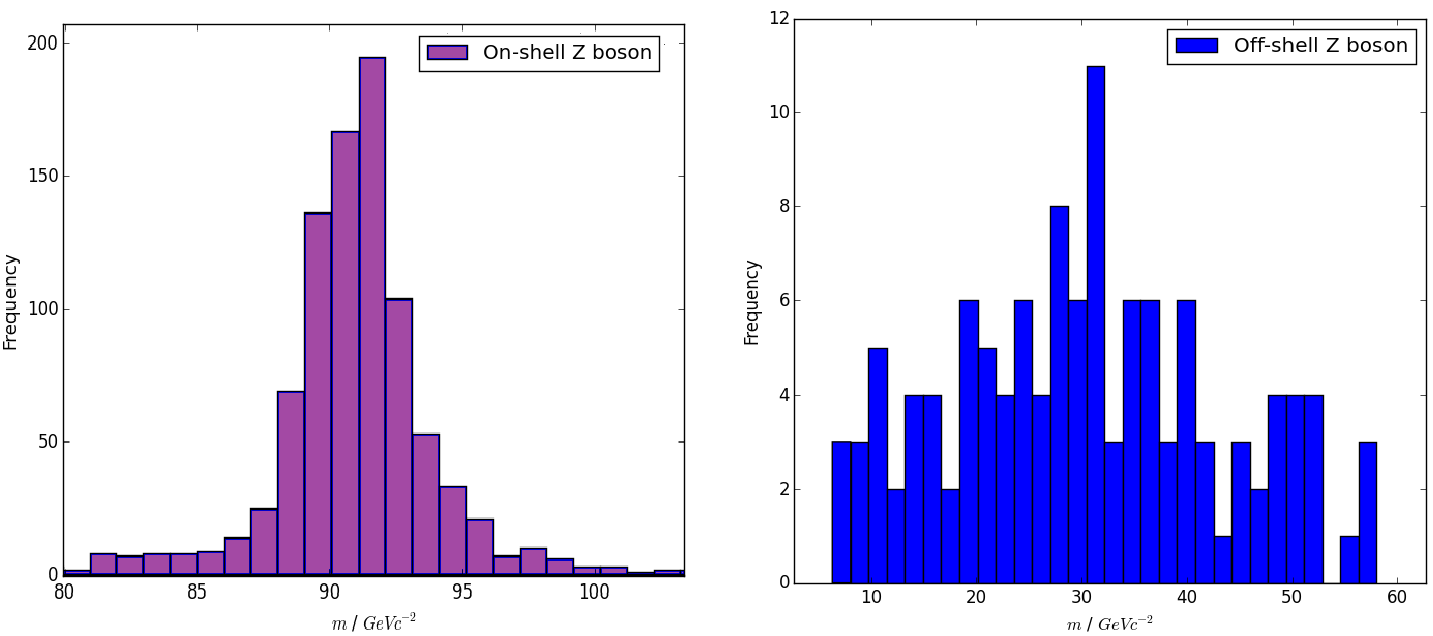
\includegraphics[width=15cm]{zbosons.png}
\caption{Histograms of the mass distributions of an on-shell and an off-shell Z boson.}
	\label{zbosons}
\end{figure}

The decay width of the on-shell $Z$ boson, i.e. the intrinsic uncertainty of its mass due to its short life-time, is about $2.5\ GeVc^{-2}$~\cite{zbosonwidth}. The off-shell boson is an even more short-lived particle and therefore its width is significantly larger. Both widths are higher than the respective statistical errors associated with the model detector systems. Hence, their detection does not significantly affect the measurement of their mass distribution and thus can be considered reliable.\\

\begin{figure}[h]
\centering
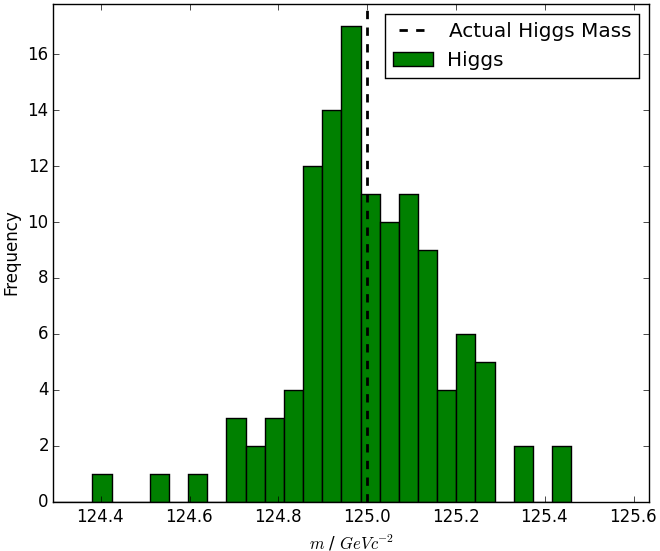
\includegraphics[width=12cm]{higgs.png}
\caption{Histogram of the mass distribution of a Higgs boson.}
	\label{higgs}
\end{figure}

The Higgs mass distribution was derived from the $Z$ boson measurements and plotted in figure \ref{higgs}. This distribution also approximates a Gaussian distribution as expected with a mean value of $124.98\ GeVc^{-2}$ with a standard error of $0.02\ GeVc^{-2}$. The decay width of the Higgs boson is approximately $6.1\ MeV$~\cite{higgswidth} which is lower than the statistical error found with the simulation. It can hence be concluded that the effective resolution of the detector systems affects the measurement of the mass distribution. Therefore, the simulation suggests that the model detector systems used to measure the Higgs boson can be improved in terms of precision.\\

The statistical error found is extremely small compared to literature values of the measured standard error which are closer to $0.4\ GeVc^{-2}$~\cite{higgsuncertainty}. There are several reasons as to why the simulation yielded more precise results than it should. Most importantly, the simulated Higgs decays were of the order of hundreds and all muons detected were assumed to be products of these decays. In reality, the confirmed Higgs decays are much fewer and there are muon products from several different sources. Other sources of error like scattering of the muons in the detectors, the inhomogeneity of the magnetic field outside the solenoid magnet and occasional failure of some detectors were not included in the model but in fact contribute to the statistical error. In this case of a higher statistical error, the Higgs boson decay width is comparatively even smaller and the resolution of the Higgs mass distribution is even more severely affected.

\section*{Conclusion}

The aim of the investigation was to compare the effective resolution of the measurements between the silicon tracker and the DT detectors in the CMS. This was done by examining the performance of the detectors in measuring muon momentum over the range of possible energy values. Making use of this analysis, the model was extended to simulate a typical Higgs boson decay which yielded results for the mass distributions of the related bosons.\\

Generally, the results suggest that the overall resolution of the detectors depends heavily on the momentum of the muons. The accuracy of the measurements from the detectors was found to be very high for momenta lower than $400\ GeVc^{-1}$. Beyond that the silicon tracker increasingly underestimated the momentum, while the DTs remained within $10\%$ of the actual value, rendering it the more reliable detection system for high momenta. The precision of the silicon tracker was found to be better for momenta lower than $80 - 100\ GeVc^{-1}$. Beyond that interval, the DT system overtakes the tracker in resolution, although both detector systems become less precise as momentum increases.

\pagebreak

The mass of the on-shell and off-shell $Z$ bosons were measured to be $(91\pm1)\ GeVc^{-2}$ and $(30\pm5)\ GeVc^{-2}$ respectively. These measurements were determined to be reliable as the statistical error associated with their detection process was lower than their intrinsic width. The mass of the Higgs boson was found to be $(124.98\pm0.02)\ GeVc^{-2}$. In this case the statistical error was higher than the Higgs boson intrinsic width, implying that the mass resolution can still be improved. The estimated error for the mass was extremely small due to the negligence of some sources of error and the unrealistically high frequency of the Higgs decay detection.\\

The simulation can be extended in various ways. Other sources of error for the detection of momentum could be included such as the ones listed in the discussion of the error in the Higgs boson mass. It would be more realistic to take into account that most of the detected muons come from sources other than Higgs decays. Other detectors like the ones perpenicular to the $z$ axis in figure \ref{cmslayout} could be taken into consideration for a more reliable prediction of the muon trajectory. A more complicated process of energy loss in the HCAL could be modelled for a more realistic simulation of the muon behaviour in the DT system. The investigation could finally be used to simulate decays other than the Higgs decay, such as pion decays~\cite{otherdecay}.

\begin{thebibliography}{1}

\bibitem {cms} The CMS Collaboration, ``The performance of the CMS muon detector in proton–proton collisions at $\sqrt{s} = 7\ TeV$ at the LHC'', JINST, March 2014.
\bibitem {zbosonwidth} Beringer J. et al, ``2012 Review of Particle Physics - Gauge and Higgs Bosons'', Physical Review Letters, 2012
\bibitem {higgswidth} Barger V. et al, ``Total Width of $125\ GeV$ Higgs Boson'', Physical Review Letters, 2012.
\bibitem {higgsuncertainty} The CMS Collaboration, ``Combination of standard model Higgs boson searches and measurements of the properties of the new boson with a mass near 125 GeV'', CMS Physics Analysis Summaries, November 2012.
\bibitem {otherdecay} The CMS Collaboration, ``Study of the inclusive production of charged pions, kaons, and protons in pp collisions at$\sqrt{s} = 0.9, 2.76, and 7\ TeV$, European Physics Journal, January 2013.
\bibitem {theory} Ragusa F., ``An Introduction to Charged Particles Tracking'', Italo-Hellenic School of Physics, 2006.
\bibitem {atlas} The ATLAS Collaboration, ``Observation of a new particle in the search for the Standard Model Higgs boson with the ATLAS detector at the LHC'', ScienceDirect, September 2012.
\bibitem {sitracker} Azzurri P., ``The CMS Silicon Strip Tracker'', IOP, 2006. 
\bibitem {cal} Garutti E., ``Calorimeters Energy measurement'', University of Hamburg, n.d.
\bibitem {cal2} Benaglia A. D., ``Measurement of the Muon Stopping Power in Lead Tungstate with the Electromagnetic Calorimeter in CMS'', IOP, 2011.

\end{thebibliography}

\end{document}
